\chapter{Weak Solutions and the Finite Element Method}

Let us consider once more our toy BVP 
\begin{equation}\label{eq:l20:toy-BVP}
    - u''(t) = f(t), \qquad t \in (0,1), \qquad u(0) = u(1) = 0.
\end{equation}
In the last lecture we introduced a spectral collocation 
method for solving this problem where we 
wrote 
\begin{equation*}
    u(t) = \sum_{n=0}^N c_n \varphi_n(t)
\end{equation*}
plugged it into the BVP and asked for zero residual on a grid. 
Further recall the hat functions $\phi_n$ that we 
introduced as well, see \Cref{fig:hat-functions}, 
\begin{equation*}
\begin{aligned}
    \phi_0(t) &= \left\{
        \begin{aligned}
            & \frac{t_1 - t}{t_1 - t_0} && t \in[t_0, t_1] \\ 
            & 0 && \text{otherwise}, 
        \end{aligned}
    \right. \\
    \phi_{n}(t)& = \left\{
         \begin{aligned}
            & \frac{t - t_{n-1}}{t_n - t_{n-1}} && t \in[t_{n-1}, t_n] \\
            & \frac{t_{n+1} - t}{t_{n+1} - t_n} && t \in[t_n, t_{n+1}] \\ 
            & 0 && \text{otherwise}, 
        \end{aligned}
    \right. \\
    \phi_N(t) &= \left\{
        \begin{aligned}
            & \frac{t - t_{N-1}}{t_N - t_{N-1}} && t \in[t_{N-1}, t_N] \\ 
            & 0 && \text{otherwise}.
        \end{aligned}
    \right.
\end{aligned}
\end{equation*}
where the middle formula defines $\phi_n$ for the interior indices 
$n = 1, \dots, N-1$. While these are natural for interpreting our piecewise linear 
interpolants on arbitrary grids, they are not suitable for 
collocation; notice that the hat functions are not differentiable 
at the grid points so we cannot just plug the expansion 
$u(t) = \sum_{n=0}^N c_n \phi_n$ into the BVP. The natural 
use case for these functions is in a different type of approach 
for solving BVPs that relies on the so-called {\it weak form}
of the problem. 

\section{Weak forms and weak solutions}
\begin{figure}[!htbp]
    \centering
    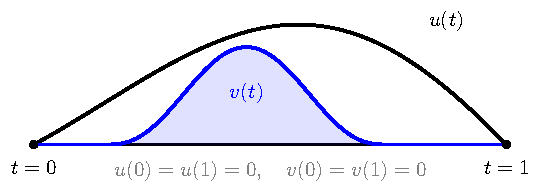
\includegraphics{./Lectures/Lec20/weak_form_cartoon.pdf}
    \caption{Cartoon of the solution $u$ and a potential 
    test function $v$ in \eqref{eq:l20:weak-form-BVP}.}
    \label{fig:weak-form-cartoon}
\end{figure}
Consider the BVP \eqref{eq:l20:toy-BVP} and multiply both sides
by an arbitrary smooth function $v(t)$ and integrate over the domain, 
\begin{equation*}
    \int_0^1 - u''(t) v(t) dt = \int_0^1 f(t) v(t) dt.
\end{equation*}
Now integrate by parts on the left side to get 
\begin{equation*}
      \int_0^1 u'(t) v'(t) dt + (u' v)\big|_{t=0} 
      - (u' v)\big|_{t=1}  = \int_0^1 f(t) v(t) dt.
\end{equation*}
If we choose $v$ so that $v(0) = v(1) = 0$, see \Cref{fig:weak-form-cartoon}, then the 
boundary terms vanish and we get 
\begin{equation}\label{eq:l20:weak-form-BVP}
    \int_0^1 u'(t) v'(t) dt = \int_0^1 f(t) v(t) dt, \qquad 
    u(0) = u(1) = 0.
\end{equation}
The above problem is called the {\it weak form of the BVP}
associated to the problem \eqref{eq:l20:toy-BVP}. In this parlance
we often refer to \eqref{eq:l20:toy-BVP} as the {\it strong form of 
the BVP}. We say that $u$ is a {\it weak solution} to the 
BVP if \eqref{eq:l20:weak-form-BVP} holds for all 
{\it test functions} $v$ that  vanish 
at the boundary.  
Once again, with this terminology, we call the solution to 
\eqref{eq:l20:toy-BVP} the {\it strong or classical 
solution to the BVP}. 

The term {\it weak} comes from the 
fact that the solution to \eqref{eq:l20:weak-form-BVP}
can be less regular than that of \eqref{eq:l20:toy-BVP}. 
Most notably, we need $u$ to be twice continuously 
differentiable to be able to impose \eqref{eq:l20:toy-BVP}
while we only need $u'$ to be square integrable to be 
able to impose \eqref{eq:l20:weak-form-BVP}. The weak formulation
above is the foundation of an important family of numerical 
solvers called the {\it Finite Element Method (FEM)}.

\section{An Encounter with the Finite Element Method}
The idea behind FEMs is to impose \eqref{eq:l20:weak-form-BVP}
for solutions $u$ of the form 
\begin{equation*}
    u(t) = \sum_{n=1}^{N-1} c_n \phi_n(t),
\end{equation*}
where we note that the hat functions from earlier are being used
and we dropped $\phi_0$ and $\phi_N$ to make sure 
$u(0) = u(1) = 0$ so that the boundary conditions 
are satisfied. 
In general we can use arbitrary basis functions $\varphi_n$ as 
well. Substituting this model into \eqref{eq:l20:weak-form-BVP}
we get 
\begin{equation}\label{eq:l20:towards-galerkin}
  \sum_{n=1}^{N-1} \int_0^1 c_n \phi_n'(t) v'(t) dt
    = \int_0^1 f(t) v(t) dt.
\end{equation}
Since we cannot impose this identity for all test functions $v$ 
we only impose it for a finite collection. A simple choice
is to take $v \in \{ \phi_1, \dots, \phi_{N-1} \}$, in which case 
\eqref{eq:l20:towards-galerkin} reduces to 
\begin{equation}\label{eq:l20:galerkin}
    \sum_{n=1}^{N-1} \int_{0}^1 c_n \phi_n'(t) 
    \phi'_j(t) dt = \int_0^1 f(t) \phi_j(t) dt, \qquad 
    \text{for } j= 1, 2, \dots, N-1.
\end{equation}
Now write $f_j = \int_{0}^1 f(t) \phi_j(t)dt$ and 
define $\fb = (f_1, \dots, f_{N-1}) \in \R^{N-1}$ as well as 
the matrix $A \in \R^{(N-1) \times (N-1)}$ with entries 
\begin{equation*}
    A_{jn} = \int_0^1 \phi'_n(t) \phi'_j(t) dt, \qquad 
    j,n \in \{1, \dots, N-1\}.
\end{equation*}
Then \eqref{eq:l20:galerkin} can be written in matrix form 
\begin{equation*}
    A \cb = \fb,
\end{equation*}
where $\cb = (c_1, \dots, c_{N-1}) \in \R^{N-1}$ is the vector of 
coefficients that define the solution $u$. Thus, we can approximate 
the solution to the weak BVP by solving the above linear system. 
The only thing that remains is for us to compute the integrals 
that define the entries $A_{jn}$ as well as the entries  
$f_j$. Noting that each $\phi_n$ is only non-zero 
in the interval $(t_{n-1}, t_{n+1})$, see \Cref{fig:hat-overlap-stiffness}, we see that 
all entries in the $j$-th row of $A$ are zero except 
\begin{equation*}
    \begin{aligned}
            A_{j, j-1} & = \int_{t_{j-1}}^{t_j} \phi'_{j-1}(t) 
            \phi'_j(t) dt\\ 
            A_{j, j}   & = \int_{t_{j-1}}^{t_{j+1}} |\phi'_{j}(t)|^2 dt \\ 
            A_{j, j+1} & = \int_{t_{j}}^{t_{j+1}} \phi'_{j+1}(t) 
            \phi'_j(t) dt,
    \end{aligned}
\end{equation*}
\begin{figure}[!htbp]
    \centering
    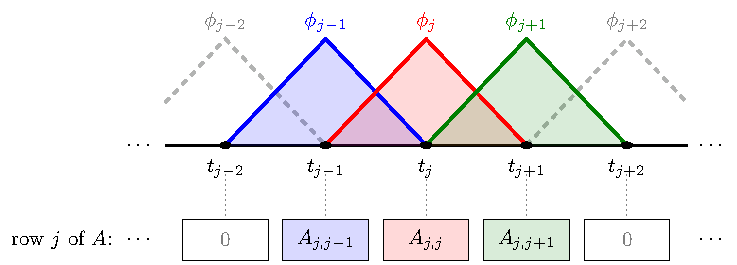
\includegraphics{./Lectures/Lec20/hat_overlap_stiffness.pdf}
    \caption{A depiction of the entries of the matrix $A$ and 
    their relation to the $\phi_n$'s. Notice that the 
    compact support of the $\phi_n$'s implies that 
    most of the entries of $A$ are zero.}
    \label{fig:hat-overlap-stiffness}
\end{figure}
with the convention that for $j=1$ we drop $A_{j, j-1}$ and for 
$j = N-1$ we ignore $A_{j, j+1}$. Since we prescribed the $\phi_j$'s we 
can compute these integrals analytically. Indeed, writing
$\Delta t_j = t_j - t_{j-1}$ for the length of the $j$-th cell, the 
derivative of each hat function is piecewise constant, 
\begin{equation*}
    \phi'_j(t) = \left\{
        \begin{aligned}
            & \frac{1}{\Delta t_j} && t \in (t_{j-1}, t_j), \\
            & -\frac{1}{\Delta t_{j+1}} && t \in (t_j, t_{j+1}), \\
            & 0 && \text{otherwise}.
        \end{aligned}
    \right.
\end{equation*}
Therefore 
\begin{equation*}
    \begin{aligned}
        A_{j, j-1} & = \int_{t_{j-1}}^{t_j} \left( -\frac{1}{\Delta t_j} \right) \frac{1}{\Delta t_j} dt
            = -\frac{1}{\Delta t_j}, \\
        A_{j, j} & = \int_{t_{j-1}}^{t_j} \frac{1}{(\Delta t_j)^2} dt 
            + \int_{t_j}^{t_{j+1}} \frac{1}{(\Delta t_{j+1})^2} dt 
            = \frac{1}{\Delta t_j} + \frac{1}{\Delta t_{j+1}}, \\
        A_{j, j+1} & = \int_{t_{j}}^{t_{j+1}} \frac{1}{\Delta t_{j+1}} \left( -\frac{1}{\Delta t_{j+1}} \right) dt
            = -\frac{1}{\Delta t_{j+1}}.
    \end{aligned}
\end{equation*}
In particular, $A$ is symmetric and tridiagonal. On a uniform grid 
with $\Delta t_j = \Delta t$ for all $j$ we obtain 
\begin{equation*}
    A = \frac{1}{\Delta t}
    \begin{bmatrix}
        2 & -1 & & & \\
        -1 & 2 & -1 & & \\
        & \ddots & \ddots & \ddots & \\
        & & -1 & 2 & -1 \\
        & & & -1 & 2
    \end{bmatrix},
\end{equation*}
which is precisely $\Delta t$ times the matrix of the second order 
centered finite difference discretization of $-u''$. To compute the 
coefficients $f_j$ we also have 
\begin{equation*}
   f_j = \int_{t_{j-1}}^{t_{j+1}} f(t) \phi_j(t)  dt,
\end{equation*}
which can be estimated using quadrature rules such as 
the trapezoidal rule or Simpson's rule. 

It is instructive to see what happens if we use the composite 
trapezoidal rule on the two cells $[t_{j-1}, t_j]$ and $[t_j, t_{j+1}]$. 
Since $\phi_j(t_j) = 1$ and $\phi_j(t_{j-1}) = \phi_j(t_{j+1}) = 0$, we get 
\begin{equation*}
    \begin{aligned}
    f_j & \approx \frac{\Delta t_j}{2} \Big( f(t_{j-1}) \phi_j(t_{j-1}) + f(t_j) \phi_j(t_j) \Big) 
    + \frac{\Delta t_{j+1}}{2} \Big( f(t_j) \phi_j(t_j) + f(t_{j+1}) \phi_j(t_{j+1}) \Big) \\
    & = \frac{\Delta t_j + \Delta t_{j+1}}{2} f(t_j).
    \end{aligned}
\end{equation*}
On a uniform grid this is simply $f_j \approx \Delta t \, f(t_j)$, and so the 
$j$-th equation of $A \cb = \fb$ reads 
\begin{equation*}
    \frac{-c_{j-1} + 2 c_j - c_{j+1}}{\Delta t^2} = f(t_j), \qquad j = 1, \dots, N-1,
\end{equation*}
with $c_0 = c_N = 0$. Furthermore, since $\phi_n(t_j) = 1$ if $n = j$ and 
$0$ otherwise, we have $u(t_j) = c_j$, i.e., the coefficients are 
precisely the values of the FEM solution at the grid points. 
Thus, with this choice of quadrature, the FEM with hat functions 
on a uniform grid reproduces exactly the second order centered 
finite difference scheme for \eqref{eq:l20:toy-BVP}. The advantage of 
the FEM point of view is that it extends naturally to non-uniform 
grids, to more accurate quadrature rules for $f_j$, and to 
higher order basis functions. 


% \bibliographystyle{plainnat}
% \bibliography{references}